\documentclass[11pt,a4paper]{article}
\usepackage[T1]{fontenc}
\usepackage[utf8]{inputenc}
\usepackage{lmodern}
\usepackage[margin=2.3cm]{geometry}
\usepackage{microtype}
\usepackage{amsmath,amssymb,mathtools}
\usepackage{booktabs}
\usepackage{multirow}
\usepackage{tabularx}
\usepackage{graphicx}
\usepackage[dvipsnames]{xcolor}
\usepackage{tikz}
\usetikzlibrary{arrows.meta,positioning,fit,calc,decorations.pathreplacing}
\usepackage{caption}
\captionsetup{font=small,labelfont=bf}
\setlength{\textfloatsep}{12pt plus 2pt minus 4pt}
\setlength{\floatsep}{10pt plus 2pt minus 2pt}
\setlength{\abovecaptionskip}{4pt}
\makeatletter\setlength{\@fptop}{0pt}\makeatother  % float-only pages start at the top
\usepackage{subcaption}
\usepackage{enumitem}
\setlist{itemsep=2pt,topsep=4pt}
\usepackage[backend=biber,style=numeric-comp,sorting=none,maxbibnames=6,minbibnames=4,giveninits=true]{biblatex}
\addbibresource{refs.bib}
\usepackage[hidelinks]{hyperref}
\usepackage[capitalise,noabbrev]{cleveref}

\definecolor{ink}{HTML}{1F2937}
\definecolor{acc}{HTML}{C2410C}
\definecolor{acc2}{HTML}{0072B2}

\newcommand{\code}[1]{\texttt{#1}}
\newcommand{\reg}[1]{\texttt{#1}}
\newcommand{\E}[2]{${#1}{\times}10^{-#2}$}  % p-value: \E{3}{247} -> 3x10^-247
\newcommand{\Eb}[2]{{#1}{\times}10^{-#2}}   % same, for use inside math
\newcommand{\weak}{\textsuperscript{w}}     % 0.001 < p < 0.05
\DeclareMathOperator{\GELU}{GELU}
\DeclareMathOperator{\clip}{clip}
\newcommand{\R}{\mathbb{R}}

\title{\bfseries Drift: a calibration-free neural decoder that adapts\\to drifting noise from its own syndromes}
\author{Chahat Patel\\[2pt]\small Symbiosis Institute of Technology, Pune}
\date{\small Whitepaper, November 2026}

\begin{document}
\maketitle

\begin{abstract}
\noindent
Error rates on quantum processors drift over time, and a decoder whose weights encode one fixed noise model
loses accuracy when the noise moves. We study a neural surface-code decoder that receives, next to each shot,
a \emph{fingerprint}: the firing rate of every detector over the last 2000 shots it has decoded. It receives no
calibration data. In circuit-level simulation ($p=0.003$) with four drift regimes, a three-seed ensemble of this
decoder at distance~5 reaches a drift-step logical error rate of 0.0457 on held-out large bursts, against 0.0980
for static matching, 0.0896 for the best sliding-window reweighted matching and 0.0426 for matching with the true
noise. With the same weights and a frozen nominal fingerprint the rate is 0.0576 (paired McNemar
$p=\Eb{3}{247}$), so the gain comes from adaptation. An auxiliary head reads hot-qubit locations from the same
inputs; it beats a training-free fingerprint score on in-distribution bursts but not, at the event level, on
held-out bursts. Three extensions with decision rules fixed in advance (multiscale and pair-covariance
fingerprints, a noise-map head with FiLM conditioning) failed those rules. All results are from simulation at
$d\le5$.
\end{abstract}

%=====================================================================
\section{Introduction}\label{sec:intro}
%=====================================================================

A surface-code memory protects one logical qubit by repeatedly measuring stabilisers and passing the resulting
detection events to a \emph{decoder}, which predicts whether the logical qubit was flipped. Most decoders depend
on a noise model: minimum-weight perfect matching (MWPM) turns error probabilities into edge weights, and a
neural decoder absorbs its training noise into its weights. On hardware the noise is not stationary. Energy-relaxation
times of superconducting qubits fluctuate in frequency and time, and two-level-system (TLS) defects are responsible
for the largest fluctuations~\cite{klimov2018fluctuations}. High-energy impacts from cosmic rays and radioactivity
cause error bursts that start at a localised impact, spread across a 26-qubit array and decay with a time constant
of about 25\,ms, occurring about every 10\,s~\cite{mcewen2022cosmic}. A decoder tuned to earlier noise then decodes
with the wrong prior, and recalibration cannot follow changes this fast.

The detection events themselves carry information about the current noise: a detector that fires more often
than usual points to a nearby error source. We ask whether a neural decoder can use this signal directly. Our
decoder receives, as a second input channel, the firing rate of every detector over the shots it has recently
decoded. It never receives calibration data or the true noise state. We call this input the fingerprint.

\paragraph{Contributions.}
\begin{enumerate}[label=(\alph*), leftmargin=2em]
  \item \textbf{A calibration-free adaptive decoder}: a small 3D convolutional decoder with a fingerprint channel and
        stale-fingerprint augmentation (\cref{sec:method}). At $d=5$ its ensemble beats static and tuned sliding-window
        MWPM on all four regimes, and MWPM with the true noise on moderate bursts and hot-qubit drift (\cref{sec:results}).
  \item \textbf{A frozen-fingerprint control}: the same weights with a fixed nominal fingerprint show that the gain
        on localised drift is adaptation, and that uniform scale drift gets almost none (\cref{sec:res-adapt}).
  \item \textbf{Drift localisation from syndromes}: an auxiliary head maps hot qubits; we compare it with a
        training-free fingerprint score and report where it is and is not better (\cref{sec:res-loc}).
  \item \textbf{Ablations with pre-set decision rules}, including negative results: richer fingerprints, a noise-map
        head with FiLM, a larger network and ensembling (\cref{sec:ablations}).
\end{enumerate}

%=====================================================================
\section{Background and related work}\label{sec:background}
%=====================================================================

\paragraph{Surface code and detection events.}
We use the rotated surface code in a $Z$-basis memory experiment with distance $d$ and $r=d$ rounds of
stabiliser measurement. A distance-$d$ patch has $d^2$ data qubits and $d^2-1$ measure qubits. Let
$m_{a,t}\in\{0,1\}$ be the outcome of stabiliser $a$ in round $t$. A \emph{detector} compares consecutive
outcomes, and a \emph{detection event} is a detector that fires:
\begin{equation}
  D_{a,t} = m_{a,t}\oplus m_{a,t-1}.
\end{equation}
Without errors every $D_{a,t}=0$. Counting the first and last layers, which contain only $Z$-type detectors, a
shot has $N=r(d^2-1)$ detectors: $N=24$ at $d=3$ and $N=120$ at $d=5$. Each shot has one label
$y\in\{0,1\}$, with $y=1$ if the logical observable flipped. A decoder maps $D\in\{0,1\}^N$ to a prediction
$\hat y$; the logical error rate (LER) is the fraction of shots with $\hat y\neq y$.

\paragraph{Matching.}
MWPM decodes on the matching graph of the detector error model. An edge $e$ with error probability $p_e$ has
weight $w_e=\ln\bigl((1-p_e)/p_e\bigr)$. We use PyMatching~2 with sparse blossom~\cite{higgott2025sparse} and
generate circuits and samples with Stim~\cite{gidney2021stim}. When the noise changes, the weights are wrong
unless they are re-estimated. Spitz et al.~\cite{spitz2018adaptive} showed that edge weights can be estimated
from the correlations of detection events, without an error model, and that the resulting adaptive decoder
works when the noise varies slowly compared with the time needed to collect those statistics. Our
sliding-window baseline (\cref{sec:setup}) is an estimator of this kind.

\paragraph{Neural decoders.}
Neural decoders can beat matching by learning correlations that matching ignores. Varbanov et
al.~\cite{varbanov2025nn} showed this on simulated and experimental small surface codes, and Lange et
al.~\cite{lange2025gnn} with a graph neural network under circuit-level noise. AlphaQubit~\cite{bausch2024alphaqubit}
pre-trained a recurrent transformer on simulated data, fine-tuned it on experimental data from Google's Sycamore
processor, and outperformed state-of-the-art decoders on that data at distances 3 and 5; AlphaQubit~2~\cite{senior2025alphaqubit2} extends the approach to larger surface and colour codes with
real-time throughput. Yan et al.~\cite{yan2026rethink} compare neural architectures under accuracy and latency
constraints and find that data scale matters more than architectural complexity at near-term distances. In these works
a decoder is matched to a noise environment by training or fine-tuning on data from it.

\paragraph{Adaptive and calibration-conditioned decoders.}
Two recent lines of work condition a decoder on information about the current device. Stein et
al.~\cite{stein2026film} encode calibration data with a graph network and condition a convolutional decoder
through feature-wise linear modulation (FiLM~\cite{perez2018film}); on IBM repetition-code experiments a single
model generalises to new qubit chains and to calibrations taken days later. Their conditioning input is the
calibration record; ours is the decoder's own syndrome history, which is available at every shot but is noisier
and lags behind the true noise. QAdapt~\cite{miao2026qadapt} adapts a neural pre-decoder across noise
environments by continual training with elastic weight consolidation. Our decoder adapts only through its input.

\paragraph{Hybrids and drift on hardware.}
Peled et al.~\cite{peled2026nmwpm} predict MWPM edge weights per syndrome with a graph network and a
transformer. Chamberland et al.~\cite{chamberland2026predecoder} use a local neural pre-decoder in front of a
global matching decoder and also infer matching weights from syndrome statistics. We do not build a hybrid here.
Hoyt et al.~\cite{hoyt2026compat} show on IBM and Google data that syndrome statistics drift away from the
stationary detector error model used for decoding, and use the mismatch for post-selection; this is evidence that
syndrome statistics drift on current hardware. The below-threshold surface-code memories on Google's Willow
processor~\cite{google2025below} are the hardware data we plan to test on next.

%=====================================================================
\section{Method}\label{sec:method}
%=====================================================================

\Cref{fig:pipeline} shows the data flow from a drifting noise state to the decoder's two input channels.

\begin{figure}[t]
\centering
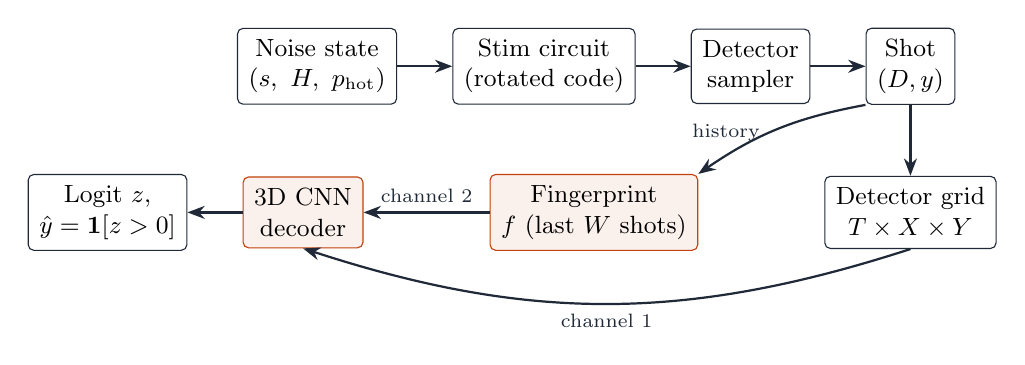
\begin{tikzpicture}[
  box/.style={draw=ink, rounded corners=2pt, align=center, font=\small, minimum height=9mm, inner sep=4pt, fill=white},
  hl/.style={box, fill=acc!8, draw=acc},
  arr/.style={-{Stealth[length=2.2mm]}, thick, ink},
  node distance=6mm and 7mm]
\node[box] (ns) {Noise state\\$(s,\ H,\ p_{\mathrm{hot}})$};
\node[box, right=of ns] (circ) {Stim circuit\\(rotated code)};
\node[box, right=of circ] (samp) {Detector\\sampler};
\node[box, right=of samp] (shot) {Shot\\$(D, y)$};
\node[box, below=9mm of shot] (grid) {Detector grid\\$T\times X\times Y$};
\node[hl, left=16mm of grid] (fp) {Fingerprint\\$f$ (last $W$ shots)};
\node[hl, left=16mm of fp] (net) {3D CNN\\decoder};
\node[box, left=of net] (out) {Logit $z$,\\$\hat y = \mathbf 1[z>0]$};
\draw[arr] (ns) -- (circ);
\draw[arr] (circ) -- (samp);
\draw[arr] (samp) -- (shot);
\draw[arr] (shot) -- (grid);
\draw[arr] (shot.south west) to[bend right=12] node[font=\scriptsize, left, pos=0.55]{history} (fp.north east);
\draw[arr] (grid.south) to[bend left=18] node[font=\scriptsize, below]{channel 1} (net.south);
\draw[arr] (fp) -- node[font=\scriptsize, above]{channel 2} (net);
\draw[arr] (net) -- (out);
\end{tikzpicture}
\caption{Data flow. The decoder never sees the noise state $(s,H,p_{\mathrm{hot}})$; it sees the current shot and
the firing rates of the shots it decoded before it.}
\label{fig:pipeline}
\end{figure}

\subsection{Noise model and drift regimes}\label{sec:noise}
The nominal circuit uses uniform circuit-level depolarising noise of strength $p_0=0.003$: two-qubit
depolarising noise after every two-qubit gate, single-qubit depolarising noise on every data qubit before every
round, and bit-flip errors after resets and before measurements. A \emph{noise state}
$\mathcal N=(s,H,p_{\mathrm{hot}})$ scales every location to $p=s\,p_0$ and adds a single-qubit depolarising
channel of strength $p_{\mathrm{hot}}$ after every circuit layer to each qubit in the set $H$ of hot qubits. Hot
qubits are always the $k$ qubits nearest to some centre, so they form a spatial cluster, as a defect or a
radiation event would. The state $(1,\varnothing,0)$ is \emph{nominal}.

A stream consists of 150 \emph{steps} of 2000 shots each; the noise state is fixed within a step and evolves between
steps according to a regime (\cref{fig:regimes}):
\begin{description}[leftmargin=1.2em, labelindent=0em, itemsep=1pt]
\item[\reg{telegraph}] global scale $s_t\in\{1,2\}$, switching with probability $0.04$ per step;
\item[\reg{hot\_qubit}] from step 50 on, the two qubits nearest the centre are hot with $p_{\mathrm{hot}}=0.03$;
\item[\reg{bursts}] when no burst is active, a burst starts with probability $0.04$; it makes the 5 qubits nearest
  to a random centre hot with $p_{\mathrm{hot}}=0.05$ for 4 steps;
\item[\reg{bursts\_big}] as \reg{bursts} with 8-qubit clusters and $p_{\mathrm{hot}}=0.1$. This regime lies outside
  the training distribution on both axes and is held out.
\end{description}
\reg{telegraph} and \reg{hot\_qubit} are simplified versions of TLS-induced fluctuations~\cite{klimov2018fluctuations}:
switching between two noise levels (here applied to the whole patch) and a persistent local defect. \reg{bursts} is a
simplified radiation event~\cite{mcewen2022cosmic}: a fixed cluster for a few steps, where the measured events spread
over the whole array. For scale, and only as a rough estimate, not a hardware claim: at roughly 1\,\textmu s per
stabiliser round, a 2000-shot window of 5-round $d=5$ experiments spans about $2000\times5\,$\textmu s $=10\,$ms plus
reset and readout overhead between shots, so of order 10\,ms, comparable to the 25\,ms decay of a cosmic-ray burst.
A fifth regime, \reg{wander} (an Ornstein--Uhlenbeck walk in $\ln s$), was evaluated only at $d=3$ on one stream and
behaved like \reg{telegraph}; we do not report it further. A \reg{static} regime (always nominal) serves as a control.

\begin{figure}[t]
\centering
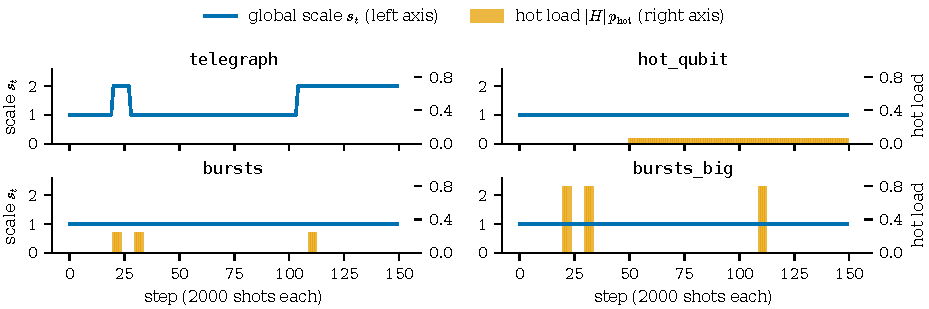
\includegraphics[width=\linewidth]{fig/regimes.pdf}
\caption{One sample schedule of each evaluated regime at $d=5$ (150 steps of 2000 shots), drawn with the same random
seed, so \reg{bursts} and \reg{bursts\_big} share burst times and differ in cluster size and $p_{\mathrm{hot}}$.}
\label{fig:regimes}
\end{figure}

\subsection{Training distribution}\label{sec:traindist}
Training never uses the regimes. Each training \emph{chunk} draws an independent noise state:
$\ln s\sim\mathcal U(\ln0.5,\ln2.5)$, and with probability $\tfrac12$ a hot cluster of
$k\sim\mathcal U\{1,\dots,6\}$ qubits around a uniformly random centre with
$p_{\mathrm{hot}}\sim\mathcal U(0.005,0.08)$; otherwise $H=\varnothing$. A chunk holds $B=512$ training shots and
$W=2000$ further shots from the same noise state, used only to compute the fingerprint. We call this the
\emph{wide} distribution. A \emph{nominal-only} dataset fixes every chunk to the nominal state.
\reg{bursts} ($k=5$, $p_{\mathrm{hot}}=0.05$) lies inside the wide range; \reg{bursts\_big} ($k=8$,
$p_{\mathrm{hot}}=0.1$) does not.

\subsection{Input and fingerprint}\label{sec:fingerprint}
Every detector has Stim coordinates $(x,y,t)$, so a shot fills a grid of shape $(T,X,Y)=(r+1,d+1,d+1)$, that is
$6\times6\times6$ at $d=5$; cells without a detector stay zero (\cref{fig:shot}). The fingerprint is the empirical
firing rate of each detector over the last $W$ shots the decoder has decoded,
\begin{equation}
  f_a = \frac{1}{W}\sum_{k=1}^{W} D^{(k)}_a,\qquad f\in[0,1]^N,\quad W=2000,
\end{equation}
laid out on the same grid and multiplied by 10 so that its values are on a scale similar to the 0/1 events. Since
$f_a$ estimates $\Pr[D_a=1]$, it reflects both the overall noise level and where the noise is concentrated
(\cref{fig:fp}). At the nominal mean firing rate of $4.27\%$ ($d=5$), the binomial standard error of one rate over
2000 shots is about $10\%$ of the rate.

\begin{figure}[t]
\centering
\begin{subfigure}{\linewidth}\centering
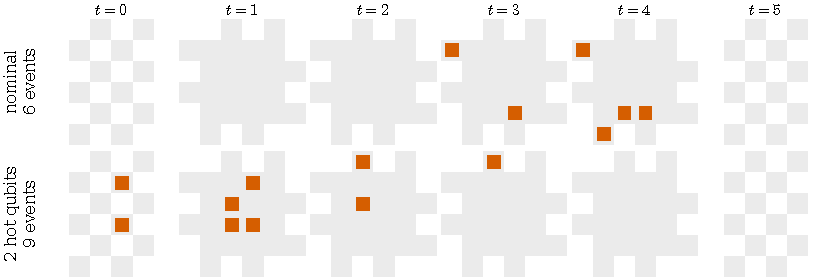
\includegraphics[width=0.9\linewidth]{fig/shot.pdf}
\caption{Two $d=5$ shots, one panel per time layer. Grey: cells that hold a detector; squares: detection events.
Top: nominal noise. Bottom: two hot central qubits.}\label{fig:shot}
\end{subfigure}\\[4pt]
\begin{subfigure}{\linewidth}\centering
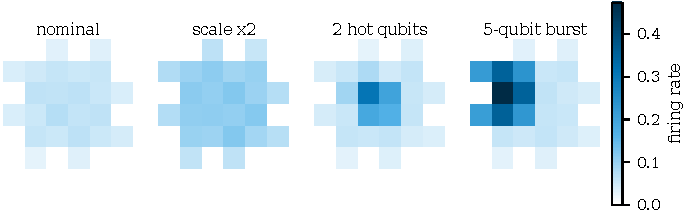
\includegraphics[width=0.84\linewidth]{fig/fingerprint.pdf}
\caption{Fingerprints ($W=2000$ shots), averaged over the four middle time layers. A global scale change raises
every rate; hot qubits and bursts raise the rates of nearby detectors only.}\label{fig:fp}
\end{subfigure}
\caption{What the decoder sees at $d=5$: the current shot (channel~1) and the fingerprint (channel~2).}
\label{fig:inputs}
\end{figure}

\subsection{Architecture}\label{sec:arch}
The decoder is a 3D convolutional network (\cref{fig:arch}). Its input is $x\in\R^{C\times T\times X\times Y}$ with
$C=1$ for a static model (the shot) and $C=2$ for an adaptive model (shot and fingerprint). With $L$ layers of
width $H_c$,
\begin{equation}
  h^{(0)}=x,\qquad h^{(\ell)}=\GELU\bigl(K^{(\ell)}*h^{(\ell-1)}+b^{(\ell)}\bigr),\quad \ell=1,\dots,L,
\end{equation}
where $K^{(\ell)}$ is a $3\times3\times3$ convolution with zero padding. The last feature map is pooled by mean
and by maximum over all grid positions, $u=[\,\mathrm{mean}_v h^{(L)}_{:,v}\,;\,\max_v h^{(L)}_{:,v}\,]\in\R^{2H_c}$,
and a two-layer head gives one logit $z=w_2^{\top}\GELU(W_1u+b_1)+b_2$ with $W_1\in\R^{64\times2H_c}$. The
decision is $\hat y=\mathbf 1[z>0]$ and the loss is binary cross-entropy. The default $H_c=48$, $L=4$ has 195\,681
parameters with a fingerprint channel and 194\,385 without; after four layers the receptive field ($9^3$) covers
the whole $d=5$ grid.

\begin{figure}[t]
\centering
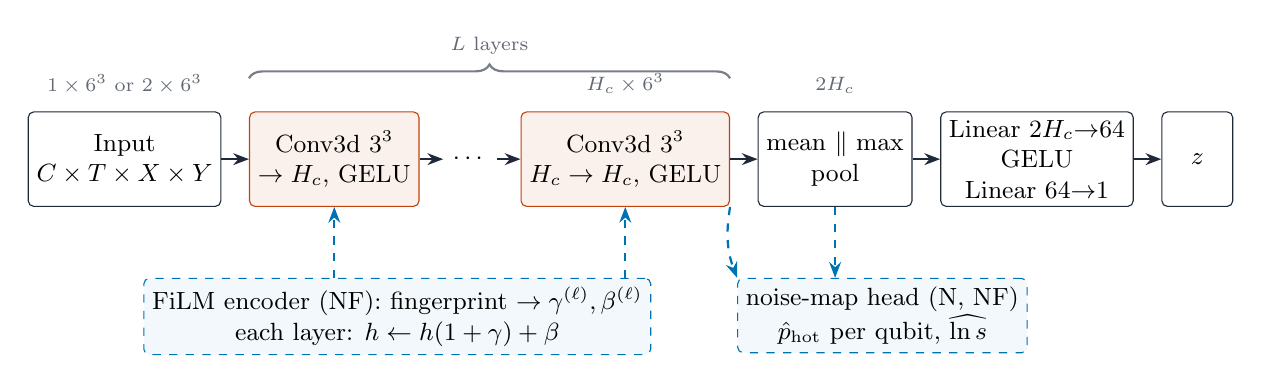
\begin{tikzpicture}[
  lay/.style={draw=ink, rounded corners=2pt, align=center, font=\small, minimum height=12mm, minimum width=16mm, fill=white, inner sep=3pt},
  hl/.style={lay, fill=acc!8, draw=acc},
  opt/.style={lay, dashed, draw=acc2, fill=acc2!5, minimum height=9mm},
  arr/.style={-{Stealth[length=2mm]}, thick, ink},
  oarr/.style={-{Stealth[length=2mm]}, thick, acc2, dashed},
  dim/.style={font=\scriptsize, text=ink!70},
  node distance=3.5mm]
\node[lay] (in) {Input\\$C\times T\times X\times Y$};
\node[hl, right=of in] (c1) {Conv3d $3^3$\\$\to H_c$, GELU};
\node[font=\small, right=3mm of c1] (dots) {$\cdots$};
\node[hl, right=3mm of dots] (cL) {Conv3d $3^3$\\$H_c\to H_c$, GELU};
\node[lay, right=of cL] (pool) {mean $\Vert$ max\\pool};
\node[lay, right=of pool] (head) {Linear $2H_c{\to}64$\\GELU\\Linear $64{\to}1$};
\node[lay, right=of head, minimum width=9mm] (z) {$z$};
\draw[arr] (in) -- (c1); \draw[arr] (c1) -- (dots); \draw[arr] (dots) -- (cL);
\draw[arr] (cL) -- (pool); \draw[arr] (pool) -- (head); \draw[arr] (head) -- (z);
\node[dim, above=1mm of in] {$1\times6^3$ or $2\times6^3$};
\node[dim, above=1mm of cL] {$H_c\times6^3$};
\node[dim, above=1mm of pool] {$2H_c$};
\draw[decorate, decoration={brace, amplitude=5pt}, thick, ink!60]
  ($(c1.north west)+(0,0.42)$) -- node[dim, above=5pt]{$L$ layers} ($(cL.north east)+(0,0.42)$);
\node[opt, below=9mm of c1, xshift=8mm] (enc) {FiLM encoder (NF): fingerprint $\to\gamma^{(\ell)},\beta^{(\ell)}$\\each layer: $h\leftarrow h(1+\gamma)+\beta$};
\node[opt, below=9mm of pool, xshift=6mm] (nh) {noise-map head (N, NF)\\$\hat p_{\mathrm{hot}}$ per qubit, $\widehat{\ln s}$};
\draw[oarr] (c1.south |- enc.north) -- (c1.south);
\draw[oarr] (cL.south |- enc.north) -- (cL.south);
\draw[oarr] (cL.south east) to[bend right=15] (nh.north west);
\draw[oarr] (pool.south) -- (pool.south |- nh.north);
\end{tikzpicture}
\caption{The decoder; shapes are for $d=5$, default $H_c=48$, $L=4$. Solid: the model used for all main results.
Dashed: the optional noise-map head (variants N and NF) and FiLM conditioning (variant NF), \cref{sec:noisehead}.}
\label{fig:arch}
\end{figure}

\subsection{Stale-fingerprint augmentation}\label{sec:stale}
In training, the fingerprint always matches the shots. At the start of a burst it does not: the window still holds
pre-burst shots. Models trained only on matching fingerprints trusted them fully and decoded badly at burst onset.
With probability $q=0.3$ per training step we therefore replace the fingerprint: with probability $\tfrac12$ by the
fingerprint of another random chunk $j$, and otherwise by the rates of a mixed window that takes its first $k$ rows
from chunk $j$ and the remaining $W-k$ from the current chunk $i$, with $k=\lfloor UW\rfloor$, $U\sim\mathcal U(0,1)$:
\begin{equation}
  f^{\mathrm{mix}}_a=\frac1W\Bigl(\sum_{n=1}^{k}D^{(j,n)}_a+\sum_{n=k+1}^{W}D^{(i,n)}_a\Bigr).
\end{equation}
The augmentation has its own random generator, so the chunk order is unchanged. We call the resulting model
\emph{adaptive-stale}, and the model without augmentation \emph{adaptive-wide}.

\subsection{Model variants and ensembles}\label{sec:variants}
\emph{static-wide} has no fingerprint ($C=1$) and is trained on the same wide chunks in the same order as
adaptive-wide, so the two differ only in the fingerprint channel. \emph{static-nominal} has no fingerprint and is
trained on nominal noise only. Every model is trained with three model seeds (0, 1, 2). An \emph{ensemble} averages
the logits of the three seeds and predicts a flip if the mean is positive; this rule was fixed before the ensemble
runs. In a live ensemble each member keeps its own fingerprint buffer.

\subsection{Noise-map head and FiLM}\label{sec:noisehead}
Variant N adds two auxiliary outputs (\cref{fig:arch}): a noise-map head on the last feature map that predicts
$p_{\mathrm{hot}}$ for each of the 49 qubits at $d=5$, and a head on the pooled vector that predicts $\ln s$. The loss is
\begin{equation}
  \mathcal L=\mathcal L_{\mathrm{BCE}}+0.1\,\mathrm{MSE}\bigl(10\,\hat p_{\mathrm{hot}},\,10\,p_{\mathrm{hot}}\bigr)
  +0.1\,\mathrm{MSE}\bigl(\widehat{\ln s},\,\ln s\bigr),
\end{equation}
with the auxiliary terms masked on steps whose fingerprint was made stale. The logit path is unchanged. Variant NF
also conditions every convolution layer on the fingerprint through FiLM~\cite{perez2018film}: a fingerprint
encoder of two 16-channel 3D convolutions produces per-layer $\gamma^{(\ell)},\beta^{(\ell)}$, initialised to zero,
and each layer's output becomes $h^{(\ell)}(1+\gamma^{(\ell)})+\beta^{(\ell)}$ after the GELU. Both variants use
stale augmentation. The noise map is read out per step as the mean over the step's shots of the head's output.

%=====================================================================
\section{Experimental setup}\label{sec:setup}
%=====================================================================

\paragraph{Data.}
All data are simulated with Stim~1.16.0 and decoded with PyMatching~2.4.0. Training datasets are listed in
\cref{tab:datasets} (\cref{app:data}). At $d=3$ models train for 60\,000 steps (two passes over 30\,000 chunks);
at $d=5$ for 300\,000 steps (two passes over 150\,000 chunks). Three fixed test sets of 200\,000 shots each (plus
2000 fingerprint shots) cover nominal noise, scale $\times2$, and two hot central qubits with
$p_{\mathrm{hot}}=0.03$. Each regime has five independent streams (stream seeds 0--4); test sets and streams are
byte-identical across all datasets of one distance.

\paragraph{Baselines.}
\emph{Static MWPM} uses nominal weights. \emph{Oracle MWPM} rebuilds the weights from the true noise state at
every step; it is MWPM with perfect noise knowledge, not an optimal decoder. \emph{WindowDEM} re-weights MWPM from
the last $w$ shots, estimating each edge probability from pairwise detector correlations in the manner
of~\cite{spitz2018adaptive}, with no access to the noise state. We run $w\in\{500,1000,2000,5000,10000\}$ and
report, for each regime and phase, the best window chosen after the fact. This favours WindowDEM.

\paragraph{Causal streaming.}
Each step's 2000 shots are processed in sub-batches of 200. A sub-batch is decoded first and only then added to
the decoder's history, so no decoder adapts to shots it is about to decode. The same rule applies to WindowDEM.

\paragraph{Phases.}
Each step is classified by its noise state: \emph{onset} is the first off-nominal step after a nominal one,
\emph{later} the other off-nominal steps, \emph{after} the first nominal step after an off-nominal one, and
\emph{nominal} all nominal steps; \emph{drift} is onset and later together. Pooled over five streams, \reg{bursts}
has 29 onset steps (33 bursts; four start directly after another), \reg{bursts\_big} 29, \reg{telegraph} 21 and
\reg{hot\_qubit} 5. LERs pool errors over all shots of a phase.

\paragraph{Frozen control.}
Every adaptive model is also run with its fingerprint fixed to the nominal one (computed from the nominal test
set's 2000 fingerprint shots). Live minus frozen measures adaptation with the weights held fixed.

\paragraph{Statistics.}
All decoders see the same shots, so the main test is the exact two-sided McNemar test. With $b$ the number of shots
only decoder A gets wrong and $c$ the number only B gets wrong,
\begin{equation}
  p=\min\Bigl(1,\ 2\sum_{i=0}^{\min(b,c)}\binom{b+c}{i}2^{-(b+c)}\Bigr).
\end{equation}
For single models we test each seed and report the largest $p$. With no multiple-testing correction we treat
$0.001<p<0.05$ as weak evidence (\weak{} in tables). McNemar measures shot noise for fixed models; variation between
training seeds appears only in the sample s.d.\ over three seeds.

\paragraph{Pre-set decision rules.}
The fingerprint variants of \cref{sec:ablations} were judged by rules written before each run. For the multiscale
and pair-covariance fingerprints: the variant's live ensemble must beat the adaptive-stale ensemble at onset or
after on \reg{bursts} or \reg{bursts\_big} with $p<0.001$, and must not be worse on later or drift steps of any regime
at $p<0.001$. For the noise-map variants: the ensemble must beat the adaptive-stale ensemble on \reg{bursts\_big}
drift steps with $p<0.001$, and must not be worse on drift or later steps of any regime or on the nominal test set at
$p<0.001$. We applied the rules as written.

%=====================================================================
\section{Results}\label{sec:results}
%=====================================================================

\subsection{Main comparison}\label{sec:res-main}
\Cref{tab:main} and \cref{fig:main} give drift-step LERs for the three-seed ensembles and the classical baselines.
At $d=5$ the adaptive-stale ensemble beats static MWPM and the best WindowDEM in every regime: all eight
paired tests have $p\le\Eb{2}{302}$, the largest being \reg{hot\_qubit} vs best WindowDEM; the other seven are too
small to represent in double precision. It beats oracle MWPM on \reg{bursts},
\reg{hot\_qubit} and \reg{telegraph} (on \reg{telegraph} through decoder quality, \cref{sec:res-adapt}). On held-out
\reg{bursts\_big}, oracle MWPM remains better by $+0.0031$ (\E{3}{14}).

Against the static-wide ensemble, trained on the same chunks without a fingerprint, the adaptive-stale ensemble is
lower on drift steps of every regime at both distances (\cref{sec:abl-ens} for how ensembling changes this margin).
Between the two adaptive ensembles (adaptive-wide minus adaptive-stale, paired), \reg{bursts} ($+0.0001$, $p=0.6$) and
\reg{telegraph} ($-0.0001$, $p=0.37$) tie, adaptive-stale is lower on \reg{bursts\_big} ($+0.0027$, \E{3.1}{19}) and
adaptive-wide is lower on \reg{hot\_qubit} ($-0.0002$, \E{6.3}{6}).

\begin{table}[t]
\centering
\footnotesize
\setlength{\tabcolsep}{4pt}
\begin{tabular}{@{}lllll@{}}
\toprule
Decoder & \reg{bursts} & \reg{bursts\_big} & \reg{hot\_qubit} & \reg{telegraph} \\
\midrule
\multicolumn{5}{@{}l}{\emph{$d=5$, 300\,000 training steps}} \\
static MWPM & 0.0439 & 0.0980 & 0.0181 & 0.0228 \\
best WindowDEM & 0.0356 & 0.0896 & 0.0108 & 0.0229 \\
oracle MWPM & 0.0197 & 0.0426 & 0.0103 & 0.0231 \\
static-wide ensemble & 0.0224 & 0.0564 & 0.0098 & 0.0175 \\
\quad single seeds & 0.0258\,$\pm$\,0.0021 & 0.0757\,$\pm$\,0.0153 & 0.0106\,$\pm$\,0.0005 & 0.0186\,$\pm$\,0.0004 \\
adaptive-wide ensemble & 0.0171 & 0.0484 & 0.0071 & 0.0164 \\
\quad single seeds & 0.0190\,$\pm$\,0.0011 & 0.0634\,$\pm$\,0.0125 & 0.0076\,$\pm$\,0.0002 & 0.0171\,$\pm$\,0.0003 \\
adaptive-stale ensemble & 0.0170 & 0.0457 & 0.0073 & 0.0164 \\
\quad single seeds & 0.0184\,$\pm$\,0.0008 & 0.0548\,$\pm$\,0.0059 & 0.0077\,$\pm$\,0.0004 & 0.0171\,$\pm$\,0.0002 \\
$\Delta$ vs static-wide ens. & $-0.0053$ (\E{4}{142}) & $-0.0107$ (\E{7}{158}) & $-0.0025$ (\E{1}{298}) & $-0.0010$ (\E{3}{29}) \\
$\Delta$ vs oracle MWPM & $-0.0027$ (\E{5}{27}) & $+0.0031$ (\E{3}{14}) & $-0.0030$ (\E{1}{224}) & $-0.0066$ ($<10^{-300}$) \\
\midrule
\multicolumn{5}{@{}l}{\emph{$d=3$, 60\,000 training steps}} \\
static MWPM & 0.1742 & 0.3778 & 0.0586 & 0.0239 \\
best WindowDEM & 0.1069 & 0.2848 & 0.0250 & 0.0237 \\
oracle MWPM & 0.0667 & 0.1937 & 0.0228 & 0.0239 \\
static-wide ensemble & 0.1049 & 0.2427 & 0.0276 & 0.0235 \\
\quad single seeds & 0.1058\,$\pm$\,0.0001 & 0.2496\,$\pm$\,0.0055 & 0.0268\,$\pm$\,0.0008 & 0.0237\,$\pm$\,0.0001 \\
adaptive-wide ensemble & 0.0713 & 0.2014 & 0.0196 & 0.0208 \\
\quad single seeds & 0.0725\,$\pm$\,0.0006 & 0.2071\,$\pm$\,0.0042 & 0.0202\,$\pm$\,0.0001 & 0.0209\,$\pm$\,0.0000 \\
adaptive-stale ensemble & 0.0720 & 0.2011 & 0.0208 & 0.0214 \\
\quad single seeds & 0.0730\,$\pm$\,0.0002 & 0.2037\,$\pm$\,0.0026 & 0.0213\,$\pm$\,0.0004 & 0.0216\,$\pm$\,0.0001 \\
$\Delta$ vs static-wide ens. & $-0.0329$ ($<10^{-300}$) & $-0.0416$ ($<10^{-300}$) & $-0.0068$ ($<10^{-300}$) & $-0.0021$ (\E{7}{102}) \\
$\Delta$ vs oracle MWPM & $+0.0053$ (\E{7}{35}) & $+0.0073$ (\E{3}{30}) & $-0.0020$ (\E{3}{66}) & $-0.0025$ (\E{5}{76}) \\
\bottomrule
\end{tabular}
\caption{Drift-step LER, pooled over 5 streams per regime (lower is better). Ensembles average the logits of model
seeds 0--2. ``Single seeds'': mean $\pm$ s.d.\ over those three seeds. Best WindowDEM is chosen per regime after
the fact. $\Delta$: adaptive-stale ensemble minus the named decoder on the same shots, exact McNemar $p$ in brackets.
$d=3$ models were trained for 5$\times$ fewer steps than $d=5$ models.}
\label{tab:main}
\end{table}

\begin{figure}[t]
\centering
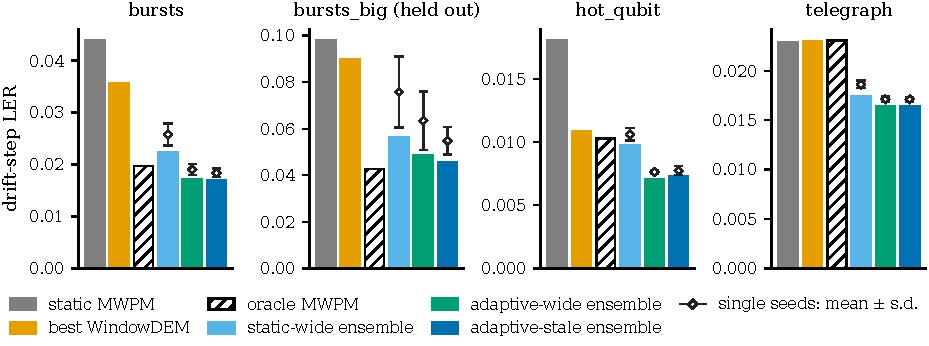
\includegraphics[width=\linewidth]{fig/main_d5.pdf}
\caption{Drift-step LER at $d=5$ per regime, pooled over 5 streams. Bars: classical baselines and three-seed
ensembles. Diamonds with error bars: mean $\pm$ sample s.d.\ of the three single-seed members of each ensemble.
Note the different $y$ scales.}
\label{fig:main}
\end{figure}

At $d=3$ the same ordering holds against static MWPM, the best WindowDEM and static-wide, but the adaptive ensembles
trail oracle MWPM on both burst regimes. Most of that remaining gap is at burst onset (adaptive-stale ensemble vs
oracle: $+0.0219$ on \reg{bursts}, \E{2}{90}; $+0.0224$ on \reg{bursts\_big}, \E{7}{59}); on later steps the
adaptive-stale ensemble ties oracle on \reg{bursts} ($+0.0006$, $p=0.2$).

\subsection{The gain is adaptation}\label{sec:res-adapt}
\Cref{fig:liveFrozen} and \cref{tab:liveFrozen} compare each adaptive ensemble with itself under a frozen nominal
fingerprint. On localised drift the live fingerprint lowers the drift-step LER in every case at $p\le\Eb{1}{209}$. At
$d=3$, frozen adaptive models are worse than static-wide: averaged over single seeds on \reg{bursts}, adaptive-wide
frozen is $+0.0253$ above static-wide ($p<10^{-300}$ in each of the 3 seeds). The network has learned to rely on the fingerprint
instead of hedging, so the whole of its gain over static-wide, and more, comes from adaptation. At $d=5$ the frozen
ensembles are close to the static-wide ensemble (\reg{bursts\_big} drift 0.0576 vs 0.0564; paired $+0.0012$, $p=0.0015$, weak), and the live
fingerprint again supplies the gain.

On \reg{telegraph} the live fingerprint contributes $0.0002$ or less at both distances; the advantage over static-wide
there is matched by the frozen model, so uniform scale drift needs no adaptation from this decoder.

\begin{table}[t]
\centering
\footnotesize
\setlength{\tabcolsep}{4pt}
\begin{tabular}{@{}lllll@{}}
\toprule
Ensemble, live $-$ frozen & \reg{bursts} & \reg{bursts\_big} & \reg{hot\_qubit} & \reg{telegraph} \\
\midrule
$d=5$ adaptive-wide & $-0.0092$ (\E{2}{315}) & $-0.0196$ ($<10^{-300}$) & $-0.0033$ ($<10^{-300}$) & $-0.0002$ (0.002\weak) \\
$d=5$ adaptive-stale & $-0.0063$ (\E{1}{209}) & $-0.0119$ (\E{3}{247}) & $-0.0025$ ($<10^{-300}$) & $-0.0002$ (0.0002) \\
$d=3$ adaptive-wide & $-0.0568$ ($<10^{-300}$) & $-0.0891$ ($<10^{-300}$) & $-0.0194$ ($<10^{-300}$) & $-0.0000$ (0.5) \\
$d=3$ adaptive-stale & $-0.0410$ ($<10^{-300}$) & $-0.0519$ ($<10^{-300}$) & $-0.0098$ ($<10^{-300}$) & $-0.0002$ (\E{2}{5}) \\
\bottomrule
\end{tabular}
\caption{Adaptation with the weights held fixed: drift-step LER of the live ensemble minus the same ensemble with a
frozen nominal fingerprint (paired McNemar $p$). \weak{}: weak evidence, $0.001<p<0.05$.}
\label{tab:liveFrozen}
\end{table}

\begin{figure}[t]
\centering
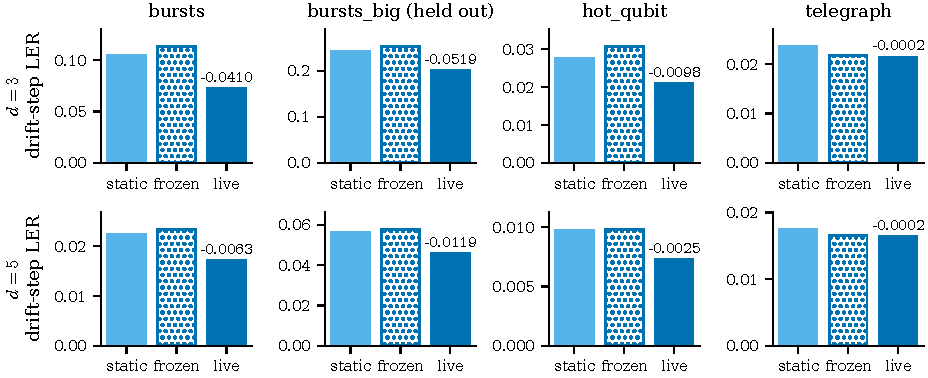
\includegraphics[width=\linewidth]{fig/live_frozen.pdf}
\caption{Live vs frozen fingerprint, adaptive-stale ensemble, drift steps. ``static'': static-wide ensemble (same
training data, no fingerprint). The number above the live bar is live $-$ frozen.}
\label{fig:liveFrozen}
\end{figure}

The live fingerprint has a cost when the noise returns to nominal: the window still holds burst shots. On the first
nominal step after a \reg{bursts\_big} event at $d=5$, the adaptive-wide ensemble is $+0.0035$ worse live than
frozen (\E{5}{41}) and $+0.0021$ worse than static MWPM (\E{3}{11}). Stale augmentation reduces the live cost to
$+0.0006$ ($p=0.0001$) and puts the adaptive-stale ensemble at $-0.0007$ against static MWPM ($p=0.006$, weak)
(\cref{fig:phases}). At $d=3$ the after-step cost is larger and stale augmentation does not remove it: the
adaptive-stale ensemble is $+0.0026$ above static MWPM after \reg{bursts\_big} events (\E{3}{13}).

The fingerprint also spares the adaptive model the cost of hedging. On the $d=3$ nominal test set, a static model
trained on nominal noise only scores 0.00536, adaptive-wide ties it (0.00532, $p=0.4$), and static-wide pays about
$13\%$ (0.00605, \E{1}{8}). At $d=5$ after 300\,000 steps this cost is not significant (largest $p=0.2$).

\subsection{Phases: onset, later, after}\label{sec:res-phases}
\Cref{fig:phases} splits the $d=5$ burst regimes by phase. On \reg{bursts} the adaptive-stale ensemble ties oracle
MWPM at onset ($-0.0001$, $p=0.9$) and beats it on later steps ($-0.0034$, \E{2}{34}). On \reg{bursts\_big} it
trails oracle at onset ($+0.0065$, \E{3}{14}) and on later steps ($+0.0019$, \E{2}{5}). WindowDEM's weakness is the
after step: its history still holds the burst, and even the best window is at 0.0116 on \reg{bursts}
against 0.0033 for static MWPM.

\begin{figure}[t]
\centering
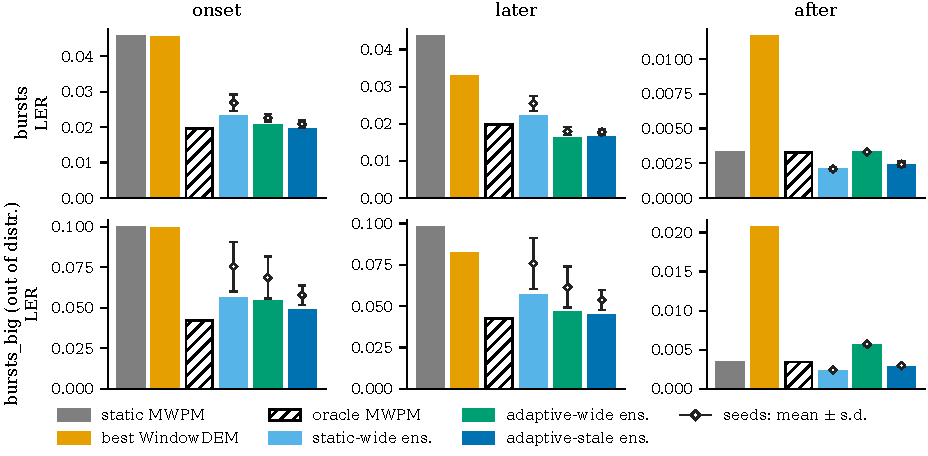
\includegraphics[width=\linewidth]{fig/phases_d5.pdf}
\caption{LER by phase on the two burst regimes at $d=5$, pooled over 5 streams (29 onset steps each). Bars as in
\cref{fig:main}. Diamonds with error bars: mean $\pm$ sample s.d.\ of the three single-seed members of each
ensemble. Best WindowDEM is chosen per phase after the fact.}
\label{fig:phases}
\end{figure}

\subsection{Training length}\label{sec:res-curves}
The $d=5$ results depend strongly on the training budget (\cref{fig:curves}, seed 0). After 60\,000 steps every
neural model lost to static MWPM on \reg{bursts\_big} drift (three-seed means 0.118 to 0.150, against 0.098), and
static-nominal was worse than MWPM on nominal noise (0.00400 vs 0.00329). After 300\,000 steps both failures are
gone in every seed (static-nominal $0.00253\pm0.00026$, largest $p=\Eb{1}{4}$). Between 240\,000 and 300\,000 steps no
seed-0 model improved on the nominal test set by more than 2 standard errors, but all five improved on
\reg{bursts\_big} drift, so the $d=5$ numbers are a snapshot of an unconverged run.

\begin{figure}[t]
\centering
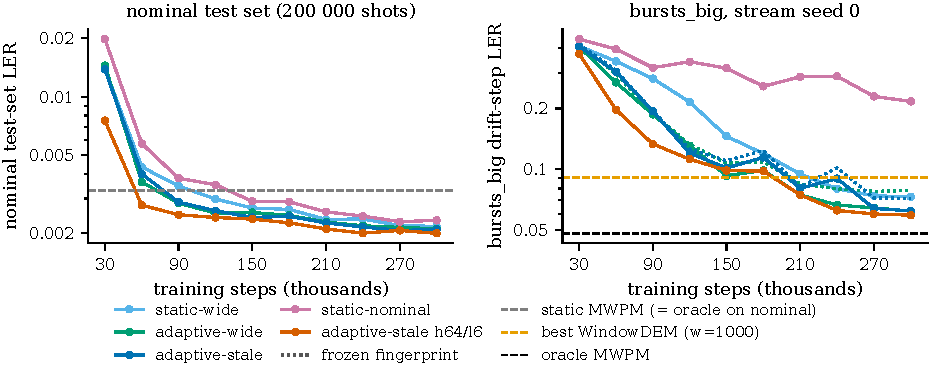
\includegraphics[width=\linewidth]{fig/curves_d5.pdf}
\caption{Learning curves at $d=5$, model seed 0 only, checkpoints every 30\,000 steps. Left: nominal test set
(log scale). Right: \reg{bursts\_big} drift steps on stream seed 0 (one stream, so single points are noisy), solid =
live fingerprint, dotted = frozen. Dashed lines: classical baselines on the same shots.}
\label{fig:curves}
\end{figure}

\subsection{Localising the drift}\label{sec:res-loc}
The NF variant's noise-map head predicts $p_{\mathrm{hot}}$ for each qubit. We score it by the top-$k$ hit rate: on a
step with $k$ truly hot qubits, the fraction of them among the $k$ qubits with the highest prediction. As a
training-free reference we score each qubit $q$ directly from the live fingerprint,
\begin{equation}
  \mathrm{score}_q=\sum_{a\in A(q)}\bigl(f_a-f^{\mathrm{nom}}_a\bigr),
\end{equation}
where $f^{\mathrm{nom}}$ is the nominal fingerprint and $A(q)$ is the set of detectors joined by a matching-graph edge
that a single-qubit Pauli fault on $q$ produces (9 to 24 detectors per qubit at $d=5$). Both methods use the same
causal 2000-shot buffer. We compare them per step and per burst event with an exact sign test; the event-level test
is the honest one, because steps within one event share hot qubits and overlapping windows.

\begin{figure}[t]
\centering
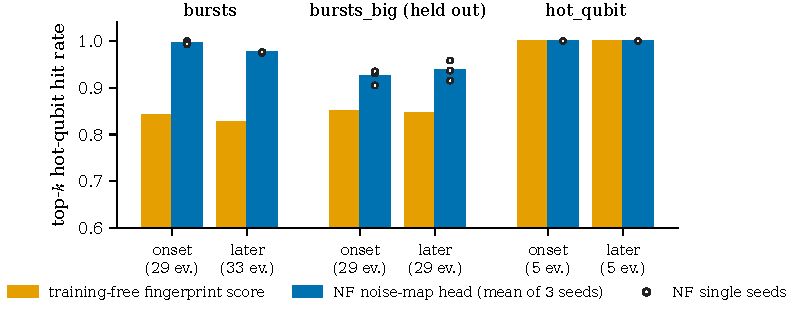
\includegraphics[width=0.72\linewidth]{fig/localisation.pdf}
\caption{Top-$k$ hot-qubit hit rate at $d=5$, pooled over 5 streams; ``ev.'' is the number of events. Orange:
training-free fingerprint score. Blue: NF noise-map head, mean of three seeds; circles: single seeds.}
\label{fig:loc}
\end{figure}

\Cref{fig:loc} shows the result. On \reg{bursts} the head is clearly better: the baseline scores 0.825 to 0.841 by
phase and NF 0.975 to 1.000 by seed and phase. Per event, NF wins 20 bursts, loses 1 and ties 12 for every seed
($p=\Eb{2}{5}$); at onset it wins 17 or 18 events and loses none ($p\le\Eb{2}{5}$). On \reg{hot\_qubit} every method,
including the training-free score, scores 1.000, so this regime cannot separate them. On held-out \reg{bursts\_big} NF
averages 0.056 to 0.114 above the baseline (0.845 to 0.849), but at the event level no seed reaches $p<0.001$; the
best cell is seed 1 on later steps ($p=0.013$, weak). The statement that the head localises held-out large bursts
better than the raw fingerprint is not supported.

The baseline's errors are near misses: 96\% (\reg{bursts}) and 100\% (\reg{bursts\_big}) of its wrong picks share a
detector with a hot qubit, and its hit rate at onset is about the same as on later steps: it loses on spatial
resolution, not reaction time. The baseline is one untuned rule, and NF's map also averages over the step's own shots.

%=====================================================================
\section{Ablations and negative results}\label{sec:ablations}
%=====================================================================

\Cref{tab:ablations} summarises the variants judged by a pre-set rule. All are three-seed ensembles compared with the
adaptive-stale ensemble on the same shots. Per-phase LERs are in \cref{app:tables}.

\begin{table}[t]
\centering
\small
\setlength{\tabcolsep}{4pt}
\begin{tabularx}{\linewidth}{@{}lllX@{}}
\toprule
Variant & $d$ & Verdict & Deciding cells (variant $-$ adaptive-stale ensemble) \\
\midrule
B: multiscale fingerprint & 3 & fails & win: \reg{bursts} onset $-0.0171$ (\E{3}{112}); loss: \reg{hot\_qubit} later $+0.0002$ ($p=0.0005$) \\
B: multiscale fingerprint & 5 & fails & win: \reg{bursts} onset $-0.0019$ (\E{2}{7}); losses: \reg{bursts\_big} drift $+0.0019$ (\E{4}{9}), later $+0.0024$ (\E{2}{11}) \\
C: B + 8 pair covariances & 3 & fails & win: \reg{bursts} onset $-0.0180$ (\E{2}{110}); losses: \reg{bursts\_big} drift $+0.0050$ (\E{8}{21}), later $+0.0082$ (\E{2}{43}) \\
N: noise-map head & 5 & fails & no win: \reg{bursts\_big} drift $+0.0007$ ($p=0.03$\weak); no losses \\
NF: noise-map head + FiLM & 5 & fails & no win: \reg{bursts\_big} drift $+0.0007$ ($p=0.04$\weak); no losses \\
\bottomrule
\end{tabularx}
\caption{Variants judged by decision rules fixed before each run (\cref{sec:setup}). C was not run at $d=5$.}
\label{tab:ablations}
\end{table}

\subsection{Multiscale fingerprint (B)}
B replaces the single fingerprint by three channels: the 2000-shot rates (long), the rates over the last 200 shots
(short), and short minus long. The short window is meant to remove the lag at burst onset.

At $d=3$ it does that. B beats the baseline at onset on \reg{bursts} ($-0.0171$, \E{3}{112}) and \reg{bursts\_big}
($-0.0175$, \E{4}{67}), and on both after steps; it ties static MWPM after bursts ($p\ge0.2$), where the baseline was
worse. It fails the rule on a single cell, \reg{hot\_qubit} later steps, by $+0.0002$ ($p=0.0005$), about 1\%
relative. We record this as a near miss and did not change the rule after the fact.

At $d=5$ the gain mostly disappears and B fails clearly. The onset gain shrinks to $-0.0019$ on \reg{bursts}
(\E{2}{7}) and is absent on \reg{bursts\_big} ($+0.0003$, $p=0.7$) and \reg{hot\_qubit} ($+0.0001$, $p=1$). B is worse on
\reg{bursts\_big} drift ($+0.0019$, $+4.1\%$, \E{4}{9}) and later steps ($+0.0024$, $+5.4\%$, \E{2}{11}), and costs
$+6.4\%$ to $+17.7\%$ relative on nominal stream steps in all four regimes ($p\le\Eb{1}{10}$), a cell the rule does not
cover. With a frozen fingerprint B and the baseline have the same nominal-step LERs, so this cost comes from the
live short channel; we have not checked the channel values. One positive result: the B ensemble beats oracle MWPM
at \reg{bursts} onset ($-0.0020$, $p=0.0002$), where the baseline tied it. The $d=3$/$d=5$ difference is confounded
with training length (60\,000 vs 300\,000 steps) and data.

\subsection{Pair-covariance channels (C)}
C adds eight pair-covariance channels to B. At $d=3$ it is the best variant on \reg{bursts} and \reg{hot\_qubit} (drift
vs baseline $-0.0064$, \E{1}{114}, and $-0.0011$, \E{2}{54}) and on the two-hot-qubit test set ($-0.00112$, \E{1}{11}),
but it is worse on \reg{bursts\_big} drift ($+0.0050$, \E{8}{21}) and much worse than B there ($+0.0112$, \E{1}{113}).
One untested explanation is that the covariance channels leave their training range under the strongest noise. It
does not explain everything: C is also worse than B on \reg{bursts\_big} with a frozen nominal fingerprint (0.2714 vs
0.2539, unpaired). C was not run at $d=5$.

\subsection{Noise-map head and FiLM (N, NF)}
Neither auxiliary head changes decoding accuracy. Both variants fail the rule because they do not improve
\reg{bursts\_big} drift; the difference is slightly positive and weak ($+0.0007$, $p=0.03$ and $p=0.04$). No cell is
worse at $p<0.001$. On the test sets NF vs the baseline is $-0.00006$ (nominal, $p=0.3$), $-0.00016$ (scale $\times2$,
$p=0.3$) and $-0.00012$ (two hot qubits, $p=0.3$). The heads are useful only as a diagnostic output (\cref{sec:res-loc}).

\subsection{Network size (h64/l6)}
A network with $H_c=64$, $L=6$ (565\,121 parameters) was trained once (seed 0, adaptive-stale). It is lower than the
seed-0 $H_c=48$, $L=4$ model on \reg{bursts\_big} drift (0.0484 vs 0.0514, $-0.0031$, \E{8}{14}) and ties it on nominal
noise ($-0.00009$, $p=0.1$), at 2.2 times the GPU time (8540\,s vs 3890\,s). It missed the pre-set adoption bar of one
percentage point on \reg{bursts\_big} drift (stream seed 0) with 0.3 points (0.0590 vs 0.0620). The three-seed $H_c=48$
ensembles (0.0457 and 0.0484) are at or below it (unpaired; one h64/l6 seed).

\subsection{Ensembling}\label{sec:abl-ens}
At $d=5$ every wide-trained ensemble beats all three of its members on drift steps of all four regimes (largest
$p=\Eb{1}{7}$); on \reg{bursts\_big} drift the gain over the best seed is $-0.0065$ (static-wide), $-0.0032$
(adaptive-wide) and $-0.0056$ (adaptive-stale). Ensembling helps static-wide more, so the adaptive-stale margin on
\reg{bursts\_big} drift falls from $-0.0209$ (single-seed mean) to $-0.0107$. It leaves live minus frozen nearly unchanged
($-0.0119$ vs a single-seed mean of $-0.0125$) and does not change the after-step cost. At $d=3$ the gains are small, and
the static-wide ensemble is worse than its best member on \reg{hot\_qubit} drift ($+0.0015$, \E{4}{137}), for reasons we
have not found.

%=====================================================================
\section{Discussion}\label{sec:discussion}
%=====================================================================

Two patterns have explanations we have not tested; we state them as hypotheses. First, the live$-$frozen gap is
largest on \reg{bursts\_big} ($d=5$ adaptive-stale ensemble: $-0.0119$, against $-0.0063$ on \reg{bursts} and $-0.0025$
on \reg{hot\_qubit}). \emph{Hypothesis:} \reg{bursts\_big} moves the noise furthest from nominal (static MWPM drift LER
0.0980, against 0.0439 on \reg{bursts}), so a nominal fingerprint misinforms the decoder most there, and a network that
never saw 8-qubit clusters cannot infer the cluster from a single shot. Second, ensembling helps static-wide more than
the adaptive models (on \reg{bursts\_big} drift, ensemble minus seed mean: $-0.0193$ for static-wide, $-0.0149$ for
adaptive-wide, $-0.0091$ for adaptive-stale). \emph{Hypothesis:} without a fingerprint each static seed must hedge over
the whole training distribution and settles on a different compromise (seed s.d.\ 0.0153, against 0.0059 for
adaptive-stale), so averaging removes more variance; the fingerprint pins down the noise state, so adaptive seeds
agree more.

%=====================================================================
\section{Limitations}\label{sec:limitations}
%=====================================================================

\begin{itemize}
  \item \textbf{Simulated drift only.} Every result comes from Stim simulations. We have not validated the decoder on
        hardware data. Google's Willow surface-code memory data~\cite{google2025below} is the planned next step.
  \item \textbf{Test regimes from the training family.} All noise is circuit-level depolarising noise with a global
        scale and hot-qubit clusters, and the test regimes come from the same family as the training data. Only
        \reg{bursts\_big} extrapolates, and only in cluster size and strength. Unseen drift types, such as correlated
        two-qubit drift, leakage, crosstalk, biased noise or coherent errors, are untested.
  \item \textbf{$d\le5$, absolute cluster sizes.} We have not tested larger codes. Cluster sizes are the same at $d=3$
        and $d=5$, so the regimes are relatively milder at $d=5$ and absolute LERs are not comparable across distances.
  \item \textbf{Latency.} MWPM is the fastest decoder we measured: in a Python benchmark on a cloud VM ($d=5$, batch 4096)
        it takes 1.85\,\textmu s per shot on CPU, the neural decoders 10.2 to 10.8\,\textmu s on an NVIDIA L4. This is not
        a real-time statement, and ensemble latency (three times the compute) was not measured. A hybrid that sets
        matching weights from the fingerprint~\cite{peled2026nmwpm,chamberland2026predecoder} could keep matching's
        speed; we have not built one.
  \item \textbf{Seeds, convergence, statistics.} Each ensemble is one trio of seeds; the learning curves and h64/l6 are
        seed 0 only. The $d=5$ \reg{bursts\_big} curves were still falling at 300\,000 steps, and $d=3$ and $d=5$ differ in
        training length as well as distance. There is no multiple-testing correction, and the best WindowDEM is chosen
        after the fact.
\end{itemize}

%=====================================================================
\section{Conclusion}\label{sec:conclusion}
%=====================================================================

A neural decoder that sees only the firing rates of its own recent detection events adapts to localised drift in
simulation. At $d=5$ its ensemble beats static and tuned sliding-window matching on every regime we tested, beats
matching with the true noise on moderate bursts and a hot-qubit defect, and trails it by $0.0031$ on held-out large
bursts. The frozen control shows the gain is adaptation. Richer fingerprints and noise heads failed their pre-set
rules. Hardware memory data, larger distances and latency are the open tests.

\section*{Code and data availability}
Code, experiment notes, result tables (Markdown, CSV, JSON) and dataset manifests with all generation seeds are at
\url{https://github.com/chahat-101/drift}. Model checkpoints, generated datasets and per-shot error bits are not in the
repository because of their size; the datasets can be regenerated from the manifests (identical samples need the same
Stim version and machine).
% TODO: decide where to host checkpoints and per-shot error bits (or state "available on request"), then update this paragraph.

\section*{AI assistance}
Code, analysis and drafting were assisted by an AI model (Claude); the author designed the study and checked all
results.

\printbibliography

\clearpage
\appendix
%=====================================================================
\section{Hyperparameters}\label{app:hyper}
%=====================================================================

\begin{table}[htbp]
\centering
\small
\begin{tabularx}{\linewidth}{@{}lX@{}}
\toprule
Setting & Value \\
\midrule
Code & rotated surface code, $Z$ memory, $d=r\in\{3,5\}$, $p_0=0.003$ \\
Detectors per shot; grid $(T,X,Y)$ & 24, $(4,4,4)$ at $d=3$; 120, $(6,6,6)$ at $d=5$ \\
Network & 3D CNN, $3^3$ kernels, GELU, $H_c=48$, $L=4$; mean$\Vert$max pool; head $2H_c\to64\to1$ \\
Parameters & 194\,385 (static), 195\,681 (adaptive); h64/l6: 563\,393 / 565\,121 \\
Fingerprint & $W=2000$ shots, scaled by 10; updated every 200 shots \\
Multiscale fingerprint (B) & long (2000 shots), short (last 200 shots), short $-$ long \\
Loss & binary cross-entropy; N/NF: $+0.1$ MSE($10\,\hat p_{\mathrm{hot}}$) $+0.1$ MSE($\widehat{\ln s}$) \\
FiLM encoder (NF) & two 16-channel 3D convolutions; zero-initialised $\gamma,\beta$ per layer \\
Optimiser & AdamW, peak learning rate $10^{-3}$, OneCycle schedule over the run \\
Batch, precision & 512 shots (one chunk) per step, fp32 \\
Training steps & 60\,000 ($d=3$); 300\,000 ($d=5$); two passes over the chunks \\
Stale augmentation & $q=0.3$; half fully stale, half mixed window \\
Model seeds; stream seeds & 0, 1, 2; 0--4 \\
Ensemble rule & mean of the three seeds' logits, flip if $>0$ \\
WindowDEM & $w\in\{500,1000,2000,5000,10000\}$; estimates clipped to $[10^{-6},0.45]$ \\
Software & Stim 1.16.0, PyMatching 2.4.0, NumPy 2.4.6, PyTorch 2.15.0 \\
\bottomrule
\end{tabularx}
\caption{Hyperparameters shared by all models unless stated.}
\label{tab:hyper}
\end{table}

%=====================================================================
\section{Datasets}\label{app:data}
%=====================================================================

\begin{table}[htbp]
\centering
\small
\begin{tabular}{@{}lllrrr@{}}
\toprule
Dataset & $d$ & Training noise & Train chunks & Train shots & On disk \\
\midrule
\code{d3\_wide} & 3 & wide & 30\,000 & 15.4\,M & $\approx0.1$\,GB \\
\code{d3\_nominal} & 3 & nominal only & 30\,000 & 15.4\,M & -- \\
\code{d5\_wide} & 5 & wide & 30\,000 & 15.4\,M & 510\,MB \\
\code{d5\_nominal} & 5 & nominal only & 30\,000 & 15.4\,M & 86\,MB \\
\code{d5\_wide\_x5} & 5 & wide & 150\,000 & 76.8\,M & 2.3\,GB \\
\code{d5\_nominal\_x5} & 5 & nominal only & 150\,000 & 76.8\,M & 393\,MB \\
\bottomrule
\end{tabular}
\caption{Training datasets. Each wide chunk has 512 training shots and 2000 fingerprint shots from one noise state;
nominal-only sets store no fingerprint shots. All have 1000 validation chunks. The 60\,000-step models used the
$30\,000$-chunk sets; the 300\,000-step $d=5$ models used the \code{\_x5} sets. Test sets (3 states $\times$ 200\,000
shots) and streams (4 regimes $\times$ 5 stream seeds $\times$ 150 steps $\times$ 2000 shots) are byte-identical within
one distance.}
\label{tab:datasets}
\end{table}

%=====================================================================
\section{Per-phase tables}\label{app:tables}
%=====================================================================

All LERs pooled over 5 streams. Ensembles of model seeds 0--2; best WindowDEM chosen per phase (window in brackets).
``--'': \reg{hot\_qubit} has no after phase.

\begin{table}[tp]
\centering
\footnotesize
\setlength{\tabcolsep}{4pt}
\begin{tabular}{@{}llllll@{}}
\toprule
Decoder & drift & onset & later & after & nominal \\
\midrule
\multicolumn{6}{@{}l}{\reg{bursts}} \\
\quad static MWPM & 0.0439 & 0.0455 & 0.0435 & 0.0033 & 0.0033 \\
\quad best WindowDEM & 0.0356 (2000) & 0.0455 (1000) & 0.0327 (2000) & 0.0116 (1000) & 0.0046 (5000) \\
\quad oracle MWPM & 0.0197 & 0.0195 & 0.0198 & 0.0033 & 0.0033 \\
\quad static-wide ens. & 0.0224 & 0.0232 & 0.0221 & 0.0021 & 0.0021 \\
\quad adaptive-wide ens. & 0.0171 & 0.0204 & 0.0162 & 0.0033 & 0.0021 \\
\quad adaptive-stale ens. & 0.0170 & 0.0194 & 0.0164 & 0.0023 & 0.0021 \\
\quad adaptive-stale ens., frozen & 0.0233 & 0.0244 & 0.0230 & 0.0019 & 0.0020 \\
\midrule
\multicolumn{6}{@{}l}{\reg{bursts\_big}} \\
\quad static MWPM & 0.0980 & 0.0993 & 0.0975 & 0.0034 & 0.0034 \\
\quad best WindowDEM & 0.0896 (2000) & 0.0992 (500) & 0.0822 (2000) & 0.0206 (500) & 0.0056 (2000) \\
\quad oracle MWPM & 0.0426 & 0.0422 & 0.0428 & 0.0034 & 0.0034 \\
\quad static-wide ens. & 0.0564 & 0.0559 & 0.0566 & 0.0022 & 0.0022 \\
\quad adaptive-wide ens. & 0.0484 & 0.0539 & 0.0466 & 0.0056 & 0.0022 \\
\quad adaptive-stale ens. & 0.0457 & 0.0487 & 0.0447 & 0.0028 & 0.0021 \\
\quad adaptive-stale ens., frozen & 0.0576 & 0.0583 & 0.0574 & 0.0022 & 0.0020 \\
\midrule
\multicolumn{6}{@{}l}{\reg{hot\_qubit}} \\
\quad static MWPM & 0.0181 & 0.0187 & 0.0180 & -- & 0.0034 \\
\quad best WindowDEM & 0.0108 (10000) & 0.0135 (5000) & 0.0108 (10000) & -- & 0.0033 (10000) \\
\quad oracle MWPM & 0.0103 & 0.0110 & 0.0103 & -- & 0.0034 \\
\quad static-wide ens. & 0.0098 & 0.0089 & 0.0098 & -- & 0.0020 \\
\quad adaptive-wide ens. & 0.0071 & 0.0073 & 0.0071 & -- & 0.0020 \\
\quad adaptive-stale ens. & 0.0073 & 0.0071 & 0.0073 & -- & 0.0021 \\
\quad adaptive-stale ens., frozen & 0.0098 & 0.0084 & 0.0098 & -- & 0.0019 \\
\midrule
\multicolumn{6}{@{}l}{\reg{telegraph}} \\
\quad static MWPM & 0.0228 & 0.0217 & 0.0229 & 0.0035 & 0.0033 \\
\quad best WindowDEM & 0.0229 (10000) & 0.0217 (10000) & 0.0230 (10000) & 0.0038 (5000) & 0.0033 (10000) \\
\quad oracle MWPM & 0.0231 & 0.0217 & 0.0232 & 0.0035 & 0.0033 \\
\quad static-wide ens. & 0.0175 & 0.0167 & 0.0175 & 0.0022 & 0.0021 \\
\quad adaptive-wide ens. & 0.0164 & 0.0154 & 0.0164 & 0.0021 & 0.0021 \\
\quad adaptive-stale ens. & 0.0164 & 0.0160 & 0.0165 & 0.0021 & 0.0021 \\
\quad adaptive-stale ens., frozen & 0.0166 & 0.0160 & 0.0167 & 0.0022 & 0.0021 \\
\bottomrule
\end{tabular}
\caption{$d=5$, 300\,000-step models.}
\label{tab:phases5}
\end{table}

\begin{table}[tp]
\centering
\footnotesize
\setlength{\tabcolsep}{4pt}
\begin{tabular}{@{}llllll@{}}
\toprule
Decoder & drift & onset & later & after & nominal \\
\midrule
\multicolumn{6}{@{}l}{\reg{bursts}} \\
\quad static MWPM & 0.1742 & 0.1792 & 0.1728 & 0.0065 & 0.0066 \\
\quad best WindowDEM & 0.1069 (2000) & 0.1143 (2000) & 0.1027 (5000) & 0.0242 (500) & 0.0093 (2000) \\
\quad oracle MWPM & 0.0667 & 0.0681 & 0.0663 & 0.0065 & 0.0066 \\
\quad static-wide ens. & 0.1049 & 0.1074 & 0.1042 & 0.0062 & 0.0062 \\
\quad adaptive-wide ens. & 0.0713 & 0.0954 & 0.0645 & 0.0133 & 0.0059 \\
\quad adaptive-stale ens. & 0.0720 & 0.0901 & 0.0669 & 0.0075 & 0.0058 \\
\quad adaptive-stale ens., frozen & 0.1130 & 0.1149 & 0.1125 & 0.0057 & 0.0057 \\
\midrule
\multicolumn{6}{@{}l}{\reg{bursts\_big}} \\
\quad static MWPM & 0.3778 & 0.3804 & 0.3769 & 0.0066 & 0.0065 \\
\quad best WindowDEM & 0.2848 (2000) & 0.2989 (1000) & 0.2760 (2000) & 0.0288 (500) & 0.0101 (2000) \\
\quad oracle MWPM & 0.1937 & 0.1926 & 0.1941 & 0.0066 & 0.0065 \\
\quad static-wide ens. & 0.2427 & 0.2416 & 0.2430 & 0.0059 & 0.0061 \\
\quad adaptive-wide ens. & 0.2014 & 0.2248 & 0.1935 & 0.0228 & 0.0062 \\
\quad adaptive-stale ens. & 0.2011 & 0.2151 & 0.1964 & 0.0092 & 0.0058 \\
\quad adaptive-stale ens., frozen & 0.2530 & 0.2514 & 0.2535 & 0.0054 & 0.0056 \\
\midrule
\multicolumn{6}{@{}l}{\reg{hot\_qubit}} \\
\quad static MWPM & 0.0586 & 0.0575 & 0.0586 & -- & 0.0067 \\
\quad best WindowDEM & 0.0250 (10000) & 0.0299 (2000) & 0.0249 (10000) & -- & 0.0066 (10000) \\
\quad oracle MWPM & 0.0228 & 0.0214 & 0.0229 & -- & 0.0067 \\
\quad static-wide ens. & 0.0276 & 0.0268 & 0.0276 & -- & 0.0061 \\
\quad adaptive-wide ens. & 0.0196 & 0.0255 & 0.0195 & -- & 0.0055 \\
\quad adaptive-stale ens. & 0.0208 & 0.0241 & 0.0208 & -- & 0.0056 \\
\quad adaptive-stale ens., frozen & 0.0307 & 0.0311 & 0.0307 & -- & 0.0057 \\
\midrule
\multicolumn{6}{@{}l}{\reg{telegraph}} \\
\quad static MWPM & 0.0239 & 0.0245 & 0.0239 & 0.0068 & 0.0064 \\
\quad best WindowDEM & 0.0237 (10000) & 0.0244 (10000) & 0.0237 (10000) & 0.0066 (10000) & 0.0064 (10000) \\
\quad oracle MWPM & 0.0239 & 0.0245 & 0.0239 & 0.0068 & 0.0064 \\
\quad static-wide ens. & 0.0235 & 0.0232 & 0.0236 & 0.0061 & 0.0060 \\
\quad adaptive-wide ens. & 0.0208 & 0.0208 & 0.0208 & 0.0055 & 0.0054 \\
\quad adaptive-stale ens. & 0.0214 & 0.0216 & 0.0214 & 0.0056 & 0.0056 \\
\quad adaptive-stale ens., frozen & 0.0217 & 0.0216 & 0.0217 & 0.0056 & 0.0056 \\
\bottomrule
\end{tabular}
\caption{$d=3$, 60\,000-step models.}
\label{tab:phases3}
\end{table}

\begin{table}[tp]
\centering
\footnotesize
\setlength{\tabcolsep}{4pt}
\begin{tabular}{@{}lllllll@{}}
\toprule
Regime & Variant & drift & onset & later & after & nominal \\
\midrule
\multicolumn{7}{@{}l}{\emph{$d=3$, 60\,000 steps}} \\
\reg{bursts} & adaptive-stale & 0.0720 & 0.0901 & 0.0669 & 0.0075 & 0.0058 \\
 & B & 0.0672 & 0.0730 & 0.0655 & 0.0061 & 0.0057 \\
 & C & 0.0655 & 0.0720 & 0.0637 & 0.0061 & 0.0057 \\
\reg{bursts\_big} & adaptive-stale & 0.2011 & 0.2151 & 0.1964 & 0.0092 & 0.0058 \\
 & B & 0.1950 & 0.1976 & 0.1941 & 0.0062 & 0.0056 \\
 & C & 0.2061 & 0.2105 & 0.2047 & 0.0068 & 0.0056 \\
\reg{hot\_qubit} & adaptive-stale & 0.0208 & 0.0241 & 0.0208 & -- & 0.0056 \\
 & B & 0.0210 & 0.0208 & 0.0210 & -- & 0.0056 \\
 & C & 0.0197 & 0.0196 & 0.0197 & -- & 0.0056 \\
\reg{telegraph} & adaptive-stale & 0.0214 & 0.0216 & 0.0214 & 0.0056 & 0.0056 \\
 & B & 0.0214 & 0.0212 & 0.0214 & 0.0058 & 0.0056 \\
 & C & 0.0212 & 0.0212 & 0.0212 & 0.0056 & 0.0056 \\
\midrule
\multicolumn{7}{@{}l}{\emph{$d=5$, 300\,000 steps}} \\
\reg{bursts} & adaptive-stale & 0.0170 & 0.0194 & 0.0164 & 0.0023 & 0.0021 \\
 & B & 0.0167 & 0.0175 & 0.0165 & 0.0020 & 0.0022 \\
 & N & 0.0169 & 0.0196 & 0.0161 & 0.0024 & 0.0021 \\
 & NF & 0.0168 & 0.0195 & 0.0161 & 0.0024 & 0.0021 \\
\reg{bursts\_big} & adaptive-stale & 0.0457 & 0.0487 & 0.0447 & 0.0028 & 0.0021 \\
 & B & 0.0476 & 0.0490 & 0.0472 & 0.0023 & 0.0022 \\
 & N & 0.0464 & 0.0500 & 0.0452 & 0.0027 & 0.0021 \\
 & NF & 0.0464 & 0.0501 & 0.0451 & 0.0029 & 0.0021 \\
\reg{hot\_qubit} & adaptive-stale & 0.0073 & 0.0071 & 0.0073 & -- & 0.0021 \\
 & B & 0.0074 & 0.0072 & 0.0074 & -- & 0.0024 \\
 & N & 0.0073 & 0.0072 & 0.0073 & -- & 0.0021 \\
 & NF & 0.0073 & 0.0070 & 0.0073 & -- & 0.0021 \\
\reg{telegraph} & adaptive-stale & 0.0164 & 0.0160 & 0.0165 & 0.0021 & 0.0021 \\
 & B & 0.0164 & 0.0158 & 0.0165 & 0.0020 & 0.0023 \\
 & N & 0.0163 & 0.0153 & 0.0164 & 0.0020 & 0.0021 \\
 & NF & 0.0163 & 0.0153 & 0.0164 & 0.0019 & 0.0021 \\
\bottomrule
\end{tabular}
\caption{Fingerprint and head variants (live ensembles of model seeds 0--2). B: multiscale
fingerprint; C: B with pair-covariance channels; N: noise-map head; NF: noise-map head with FiLM.}
\label{tab:variants}
\end{table}

\end{document}
